
\documentclass[10pt,fleqn, twocolumn]{IEEEtran}
\usepackage{amsfonts}
\usepackage{amsthm}
\usepackage{amssymb}
\usepackage{amsmath}
\usepackage{graphicx}
\usepackage{fancyhdr}


\newtheorem{Prop}{Proposition}
\newtheorem{lemma}{Lemma}
\newtheorem{theorem}{Theorem}

\setlength{\parindent}{3em} \setlength{\oddsidemargin}{0in}
\setlength{\textwidth}{6.5in} % sets 1in left and right margins
\setlength{\topmargin}{0.20in} % change to 0.2in for regular latex
%\setlength{\headheight}{0in}
%\setlength{\footheight}{0.5in}
\setlength{\footskip}{0.5in}
\setlength{\textheight}{9.0in} %sets 1in top and bottom margins
\renewcommand{\baselinestretch}{1} %set to 1.5 for double spacing.

\newcommand{\br}{{\mathbf r}}
\newcommand{\bA}{{\mathbf A}}
\newcommand{\ba}{{\bf a}}
\newcommand{\bb}{{\bf b}}
\newcommand{\bc}{{\bf c}}
\newcommand{\bC}{{\bf C}}
\newcommand{\bd}{{\bf d}}
\newcommand{\be}{{\bf e}}
\newcommand{\bE}{{\bf E}}
\newcommand{\bbf}{{\bf f}}
\newcommand{\bF}{{\bf F}}
\newcommand{\bh}{{\bf h}}
\newcommand{\bH}{{\bf H}}
\newcommand{\bg}{{\bf g}}
\newcommand{\bG}{{\bf G}}
\newcommand{\bq}{{\bf q}}
\newcommand{\bs}{{\bf s}}
\newcommand{\bm}{{\bf m}}
\newcommand{\bn}{{\bf n}}
\newcommand{\bu}{{\bf u}}
\newcommand{\bv}{{\bf v}}
\newcommand{\bw}{{\bf w}}
\newcommand{\bx}{{\bf x}}
\newcommand{\by}{{\bf y}}
\newcommand{\bz}{{\bf z}}
\newcommand{\bL}{{\bf L}}
\newcommand{\bM}{{\bf M}}
\newcommand{\bN}{{\bf N}}
\newcommand{\bS}{{\bf S}}
\newcommand{\bT}{{\bf T}}
\newcommand{\bD}{{\bf D}}
\newcommand{\bX}{{\bf X}}
\newcommand{\bP}{{\bf P}}
\newcommand{\bQ}{{\bf Q}}
\newcommand{\bI}{{\bf I}}
\newcommand{\bR}{{\bf R}}
\newcommand{\bU}{{\bf U}}
\newcommand{\bV}{{\bf V}}
\newcommand{\bW}{{\bf W}}
\newcommand{\bY}{{\bf Y}}
\newcommand{\bZ}{{\bf Z}}
\newcommand{\bJ}{{\bf J}}
\newcommand{\bB}{{\bf B}}
\newcommand{\bzero}{{\bf 0}}
\newcommand{\bgamma}{{\mbox {\boldmath $\gamma$}}}
\newcommand{\btheta}{{\mbox {\boldmath $\theta$}}}
\newcommand{\bvartheta}{{\mbox {\boldmath $\vartheta$}}}
\newcommand{\bDelta}{{\mbox {\boldmath $\Delta$}}}
\newcommand{\bLambda}{{\mbox {\boldmath $\Lambda$}}}
\newcommand{\bPsi}{{\mbox {\boldmath $\Psi$}}}
\newcommand{\bPhi}{{\mbox {\boldmath $\Phi$}}}
\newcommand{\bcA}{{\mbox {\boldmath ${\cal A}$}}}
\newcommand{\bcB}{{\mbox {\boldmath ${\cal B}$}}}
\newcommand{\bcC}{{\mbox {\boldmath ${\cal C}$}}}
\newcommand{\bcD}{{\mbox {\boldmath ${\cal D}$}}}
\newcommand{\bcF}{{\mbox {\boldmath ${\cal F}$}}}
\newcommand{\bcG}{{\mbox {\boldmath ${\cal G}$}}}
\newcommand{\bcL}{{\mbox {\boldmath ${\cal L}$}}}
\newcommand{\bcN}{{\mbox {\boldmath ${\cal N}$}}}
\newcommand{\bcR}{{\mbox {\boldmath ${\cal R}$}}}
\newcommand{\bcS}{{\mbox {\boldmath ${\cal S}$}}}
\newcommand{\bcH}{{\mbox {\boldmath ${\cal H}$}}}
\newcommand{\bcI}{{\mbox {\boldmath ${\cal I}$}}}
\newcommand{\bcO}{{\mbox {\boldmath ${\cal O}$}}}
\newcommand{\bcP}{{\mbox {\boldmath ${\cal P}$}}}
\newcommand{\bcQ}{{\mbox {\boldmath ${\cal Q}$}}}
\newcommand{\bcV}{{\mbox {\boldmath ${\cal V}$}}}
\newcommand{\bcW}{{\mbox {\boldmath ${\cal W}$}}}


\title{MIMO Relay with Finite-Rate Feedback and Imperfect Channel Estimation}
\author{Byung K. Yi\\LGE Mobile Research, San Diego, CA 92131}
\date{}
\begin{document}
\maketitle
\begin{abstract}\small
We investigate how finite-rate feedback and imperfect channel
estimation affect the performance of MIMO relay network in this
paper. We start from multi-antenna transceiver with random
beamforming and formulate the SNR and capacity loss due to channel
estimation and quantization errors. We thereafter extend the
analysis to multi-antenna relay network with multiple MIMO relay
nodes and discuss how the end-to-end throughput is scaled by MIMO
pilot size, codebook size, relay network size and inter-beam
interference. Computer simulations are also provided to
demonstrate our results.
\end{abstract}
\section{Introduction}
Multi-antenna systems have received much attention for the past
decade or so, due to their promise of higher spectrum efficiency
with no transmit power increase. Combining multi-antenna
transceiver with relay network is essential not only to provide
comprehensive coverage but also to help relieve co-channel
interference in existing wireless systems. For multiple-input
multiple-output (MIMO) transmission, it is well-known that their
performance and complexity can be improved by making channel state
information (CSI) available at the transmitter. This is usually
achieved through a special reverselink CSI feedback channel from
receiver, e.g., there is R-CQI channel for CSI feedback in UMB
(Ultra Mobile Broadband), the 4G standard by 3GPP2. In practice,
the CSI received by the transmitter is not perfect and suffers
from various impairments and limitations that include round-trip
delay, channel estimation errors, limited codebook, etc. Therefore
the actual link throughput is degraded. This kind of degradation
is more serious if the end-to-end capacity is considered for a
multi-hop MIMO relay network.

MIMO beamforming with quantized feedback has intensively been
investigated since 1990s~\cite{Gerlach94}. MIMO channel
quantization as well as codebook design in general is a Voronoi
decomposition problem, which is NP-hard. The Voronoi region for a
uniform random codebook is known to be upper-bounded by the
disk-covering problem solution and lower-bounded by the
sphere-packing problem solution. These two are open problems too.
MISO/MIMO beamforming systems have intensively been investigated
with perfect CQI Lloyd vector quantization (VQ)~\cite{Narula98},
different channel model~\cite{Mukka03} and different performance
metrics~\cite{PXia04,Roh04}. It is linked to Grassmannian line
packing problem by~\cite{Love02}. However, most of existing work
is done without considering pilot design and channel estimation
errors, even though they are among the most important components
of actual multi-antenna systems. In reality, MIMO CSI is estimated
by forwardlink common pilot channels sent from transmitter. An
overview of pilot-assisted transmission (PAT) including pilot
placement and channel estimation can be found in~\cite{Tong04}. In
most multi-antenna systems, pilot channels are designed to be
orthogonal to other channels and periodically sent by transmitter.
Nonorthogonal pilot design like superimposed pilots has recently
received much attention for channel estimation
too~\cite{Coldrey06}. Optimal pilot placement was investigated
in~\cite{Dong02}. In practical system design, it is important to
understand how MIMO pilot pattern and codebook design affect
system throughput, what is the achievable balance between them,
etc. And these problems become more critical when a multi-hop MIMO
relay network with beamforming is considered.

It is known that there is no simple solution to optimal MIMO
channel quantization and codebook design. In this paper, a
heuristic Voronoi boundary, Hamming boundary, is presented with
the concept of Hamming bound. This heuristic boundary can be taken
as a tradeoff between disk-covering circle and sphere-packing
boundary and they all asymptotically converge when the codebook
size is large. With the Hamming boundary for channel quantization,
the SINR degradation of MIMO beamforming due to channel
quantization is then formulated and discussed. Besides this,
Cramer-Rao lower bounds (CRLB) on MIMO channel estimation with
time-multiplexed pilots (TMP) and SIP are also presented and
discussed. It is shown that channel estimation error affects the
accuracy of both channel quantization and transmit power
allocation. We then extend our work to MIMO beamforming relay
network and discuss the scalability of MIMO beamforming by
codebook size, pilot size, relay network size, etc. We shows that
multi-antenna relay network with imperfect channel estimation and
quantization becomes interference-limited in high SNR region.
\section{System Model And Problem Description\label{MIMO_system_model}}
Consider a MIMO link consisting of a transmitter with $M$ transmit
antennas, a receiver with $N$ receive antenna and a MIMO channel
represented by the $N\times M$ matrix $\bH=\left[\bh_{1}\ \bh_{2}\
\ldots\ \bh_{N}\right]^{\rm T}$ with $\bh_{n}=\left[h_{n,1}\
h_{n,2}\ \ldots\ h_{n,M}\right]^{\rm T}$ . The $N\times 1$
received signal $\by$ is
\begin{equation}
\begin{array}{rcccl}
\by&=&\left[y_{1}\ y_{2}\ \ldots\ y_{N}\right]^{\rm T}& = &
\bH\bW\bx+\bn
\end{array}\label{Direct_MIMO}
\end{equation}
\noindent where $\bx=\left[x_{1}\ x_{2}\ \ldots\ x_{M}\right]^{\rm
T}$ is the $M\times 1$ signal vector transmitted by the source
with $\bR_{\bx}=\mbox{E}\left\{\bx\bx^{\rm
H}\right\}=\frac{P}{M}\bI_{M}$, $P$ is the total transmit power,
$\bW=\left[\bw_{1}\ \bw_{2}\ \ldots\ \bw_{M}\right]$ is a $M\times
M$ MIMO beamforming precoding matrix with
$\left\|\bw_{m}\right\|_2=1$, $\bn\sim{\bcC\bcN}(0,
\sigma^2\bI_{N})$ is a complex circular white Gaussian vector,
$\left[\ast\right]^{\rm T}$ and $\left[\ast\right]^{\rm H}$
denotes the transport operation and Hermitian conjugate operation,
respectively. It is known that the achievable MIMO channel
throughput or efficiency is~\footnote{Without loss of the
generality, the channel bandwidth is normalized to be $1$ in this
paper. }
\begin{equation}%\hspace{-0.2in}
\begin{array}{rcl}
\eta &=& \log\left|\bI_{N}+\frac{P}{M}\bH\bW\bW^{\rm H}\bH^{\rm
H}\right|\\
& =& \sum\limits_{k=1}^{K}\log\left(1+\frac{\rho_{i}}{M}\right)
\end{array}\label{spectral_eff}
\end{equation}
\noindent where $\rho_{i}$ denotes the received signal-to-noise
ratio (SNR) of the $k$th beam, which is given by
\begin{equation}
\begin{array}{rcccl}
\rho_{i}&=&\frac{\mbox{var}\left\{\bH\bw_{i}x_{i}\right\}}{\sigma^2}&=&\frac{\lambda_{i}P_{i}}{\sigma^2}
\end{array}\label{SNR_i}
\end{equation}
\noindent with $\lambda_{i}$ denoting the antenna gain of the
$i$th beam and also the $i$th eigenvalue of the MIMO channel
autocorrelation matrix $\bR_{\bH}$ defined by
\begin{equation}
\begin{array}{l}
\bR_{\bH}=\bH^{\rm H}\bH=\sum\limits_{m=1}^{M}\bh_{m}\bh_{m}^{\rm
H}=\sum\limits_{i=1}^{M}\lambda_{m}\bv_{i}\bv_{i}^{\rm H}
\end{array},\label{R_h}
\end{equation}
\noindent $\bv_{i}$ denotes the $i$th eigenvector, the operator
$\left|\ast\right|$ denotes the determinant of matrix $\ast$, and
$\mbox{var}\left\{\ast\right\}$ denotes the variance of random
variable $\ast$. Equation (\ref{spectral_eff}) and (\ref{SNR_i})
are the results from the assumption of perfect CSI available at
transmitter. This is the case in practical applications.
\begin{figure}
\center{
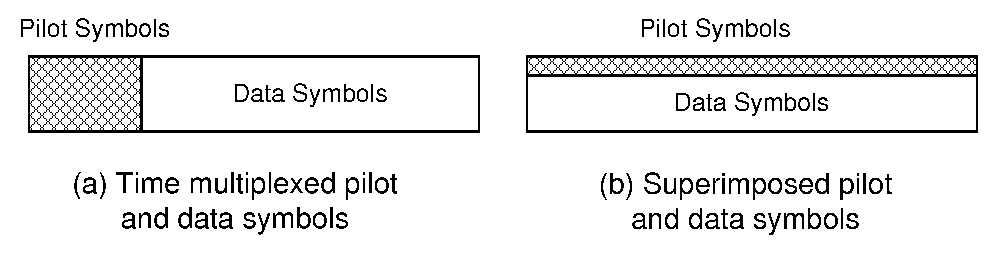
\includegraphics[width=3in, angle=0]{Pilot_Patterns.eps}
\caption{Pilot patterns for channel
estimation.}\label{pilot_pattern} }
\end{figure}
In reality, the receiver estimates channel $\bH$ or $\bR_{\bH}$
with the pilots sent by transmitter. Accuracy of the channel
estimator depends on the pilot design and placement. There are two
popular pilot patterns, TMP and SIP, received much attention for
MIMO channel estimation, which are shown in
Fig.~\ref{pilot_pattern}. TMP is a typical example of orthogonal
pilot design where pilot symbols and data symbols are separated in
both time and frequency domain, which make them orthogonal to each
other. In orthogonal pilot design, the channel estimation and data
demodulation can be done separately which may lead to simple
receiver design~\cite{Dong02}. However, SIP does the opposite. In
SIP design, where pilot and data symbols share the same time
period and frequency band and nonorthogonal to each other. In this
case, joint channel estimation/demodulation and demodulation with
pilot interference cancellation are among the most popular
receiver designs~\cite{Coldrey06}. After channel estimation,
receiver will choose a beamforming vector from a shared MIMO
precoding codebook. This is called channel quantization. And the
receiver then feeds back the chosen precoding index(es) to the
transmitter for the next transmission instead of the estimated
channel response with the assumption that the channels is not
changing fast. A MIMO codebook $\bcW$ of the size $2^B$ consisting
of $M$-dimensional normalized vectors $\left\{\bw_{1}, ...,
\bw_{2^{B}}\right\}$ is considered here. It usually takes the
receiver to feedback $B$ bits for each beam stream. A codebook is
usually designed to quantize channel responses with certain
distortion measures~\cite{Narula98}. This procedure is related to
Grassmannian line packing and spherical packing on unit sphere
$\bcS_{n}\left(1\right)$~\cite{conway96packing}, where
$\bcS_{n}(R)=\left\{\bv:\ \left\|\bv\right\|=R\right\}$ denotes
$(n-1)$-sphere of radius $R$. When a codeword $\bw_k$ is chosen to
precode transmit signals for $i$th beam $\bv_{i}$ at the
transmitter side, usually some degradation will happen on the
signal received by receiver because of imperfect channel
estimation and finite-rate feedback. This degradation on received
signals can be expressed by
\begin{equation}
\begin{array}{rcl}
\delta_{i} & = & \min\limits_{\bw\in\bcW}\left\|\bH\bv_{i}-\bH\bw\right\|\\
&=&\lambda_{i}\left(1-\bv_{i}^{\rm
H}\bw_k\right)-\sum\limits_{j\neq i}\lambda_{j}\bv_{j}^{\rm
H}\bw_{k}
\end{array}\label{delta_i}
\end{equation}
\noindent where $\bv_{i}$ is the ideal precoding vector for $i$th
eigen-mode of $\bH$. It is known that $\delta_{i}$ is one of the
major factors limiting closed-loop MIMO beamforming throughput,
which depends on $\bv_{i}$, $\bw_{k}$ and $\lambda_{i}$, etc.
There are two components in (\ref{delta_i}). The first term is
\begin{equation}
\begin{array}{rcccl}
\Delta&=&\lambda_{i}\left(1-\bv_{i}^{\rm
H}\bw_k\right)&=&\left(1-\alpha_{i}\right)\lambda_{i}
\end{array},
\end{equation}
\noindent which denotes the degradation of antenna gain, where
\begin{equation}
\begin{array}{rcl}
\alpha_{i}&=&\bv_{i}^{\rm H}\bw_k
\end{array}.\label{alpha}
\end{equation}
\noindent The second term is
\begin{equation}
\begin{array}{rcccl}
I_{} & = & \sum\limits_{j\neq i}\lambda_{j}\bv_{j}^{\rm
H}\bw_{k}&=&\sum\limits_{j\neq i}\alpha_{j}\bw_{k}
\end{array}\label{IBI}
\end{equation}
\noindent denoting inter-beam interference (IBI) due to the
correlation between $\bw_{k}$ and other eigen-modes $\bv_{j}$,
$j\neq i$. The average received signal-to-noise/interference ratio
(SINR) for the $i$th eigen-mode with the codeword $\bw_{i}$ can be
written by
\begin{equation}
\begin{array}{rcl}
\bar\rho_{i}&=&\mbox{E}_{\bv_{i}\in{\cal
V}_{k}}\left\{\frac{\lambda_{i}\left(\bv_{i}^{\rm
H}\bw_{k}\right)^2P_{i}}{n_{0}^2+ \lambda_{i}\sum\limits_{l\neq
i}^{K}\left(\bv_{i}^{\rm H}\bw_{l}\right)^{2}P_{l}}\right\}\\
&=&\mbox{E}_{\bv_{i}\in{\cal
V}_{k}}\left\{\frac{\alpha_{i}^{2}\rho_{i}}{1+
\lambda_{i}\sum\limits_{l\neq
i}^{K}\frac{\alpha_{l}^{2}}{\lambda_{l}}\rho_{l}}\right\}\ ,
\end{array}
\end{equation}
\noindent where $K\leq\mbox{min}\left\{M,\ N\right\}$ denotes the
number of beams in use.

The achievable throughput of MIMO beamforming depends on not only
the chosen precoding vectors $\bW$ but also the power distribution
$P_{k}$, $k=1,\ 2,\ \ldots,\ K$. There are many power allocation
strategies for assigning transmit power to beams with different
performance metrics. When maximizing MIMO throughput is a major
concern, the so-called water-filling strategy can be used so that
$P_{k}$ satisfies
\begin{equation}
\begin{array}{l}
P_{k}=\left(\mu-\frac{\sigma_{n}^2}{\lambda_{k}}\right)^{+}=
\begin{cases}
\mu-\frac{\sigma_{n}^2}{\lambda_{k}} & \mu-\frac{\sigma_{n}^2}{\lambda_{k}} >0 \\
0 & \mu-\frac{\sigma_{n}^2}{\lambda_{k}} < 0
\end{cases}
\end{array}
\end{equation}
with $\mu$ chosen so that the total power constraint is satisfied
\begin{equation}
\begin{array}{rcl}
\sum\limits_{k=1}^{K}P_{k}&=&P
\end{array}.\label{power_constraint}
\end{equation}
\noindent If the delay-limited power allocation strategy is used,
then
\begin{equation}
\begin{array}{rcl}
P_{k}&=&\frac{\mu}{\lambda_{k}}
\end{array}
\end{equation}
with $\mu$ chosen to satisfy (\ref{power_constraint}). This is
also called channel inversion strategy. Another simple but popular
strategy for allocating transmit power is to assign each beam the
average power so that
\begin{equation}
\begin{array}{rcl}
P_{k}&=&\frac{P}{K}
\end{array}.\label{P_aver}
\end{equation}
\noindent In the following sections, we will discuss how the
channel quantization error and imperfect channel estimation affect
the received SINR and channel capacity.
\section{Hamming Bound on Channel Quantization}
\begin{figure}
\center{
\includegraphics[width=2.40in, angle=0]{Voronoi_Bounds.eps}
\caption{Voronoi cell and various bounds}\label{Voronoi_bound} }
\end{figure}
It is known that the performance of channel quantization depends
on the Voronoi cell for each codeword. If the Voronoi
decomposition for the codebook is known, the statistic of the
correlation ratio $\alpha_i$, $i=1,\ 2,\ \ldots,\ K$ defined in
(\ref{alpha}) can be calculated. The same to the SINR $\rho_{i}$.
However, the closed-form expression of a general Voronoi cell
boundary, which is a polytope, is an open-problem even for regular
Voronoi tessellation. This makes it difficult in obtaining some
insight of the average SINR as well as achievable throughput for
each eigen-mode beamforming. There are some other problems related
to the Voronoi decomposition problem. Among them, two problems are
well-known. The first problem is called disk-covering problem in
which, given a unit disk, the problem is to find the smallest
radius for $n$ equal disks to completely cover the unit disk. The
other one is sphere-packing problem which concern arrangements of
non-overlapping identical spheres to fill a space. The
relationship between Voronoi cell and the solutions to
disk-covering problem and sphere-packing problem is illustrated in
Fig.~\ref{Voronoi_bound}. Basically sphere-packing solution gives
a lower-bound approximation of Voronoi cell and disk-covering
solution present a upper-bound approximation of it. However, these
two problems are still open in general. Instead of finding the
exact boundary for the Voronoi cell $\bcV_{i}$, we suggest another
heuristic approach, in which we use a sphere cap to approximate
the actual polytope boundary by approaching Hamming bound. This is
similar to sphere packing. However, all spheres are
non-overlappedly placed with sphere-packing. With our approach,
the interior of each sphere cap has the same area as the Voronoi
cell and they are overlapped with each other in space. The border
of this sphere cap is termed Hamming boundary. The relationship
between Hamming boundary and Voronoi cell is also shown in
Fig.~\ref{Voronoi_bound}.

With the concept of Hamming bound, the sum of sphere-cap areas is
the same as the area of the codebook sphere, which is also same to
the sum of Voronoi-cell areas. For an uniform random codebook of
size $2^{B}$ in $M$-dimensional Euclid space, the area of a
Voronoi cell is given by
\begin{equation}
\begin{array}{rcl}
A\left(\bcV_{k}\right)&=&
\frac{2{\pi}^{M}}{2^{B}\Gamma\left(M\right)}
\end{array}\label{V_area}
\end{equation}
\noindent where $\Gamma\left(\ast\right)$ denotes the gamma
function. On the other hand, the area of $(m-1)$-complex sphere
cap $\bcC_{m}^{\rm c}\left(\psi,\ R\right)$ with contact angle
$\psi$ and radius $R$ is
\begin{equation}%\hspace{-0.22in}
\begin{array}{l}
A\left(\bcC_{m}^{\rm c}\left(\psi,\
R\right)\right)=\left[1-\cos^{(2m-2)}\left(\psi\right)\right]S_{m}^{\rm
c}\left(R\right),
\end{array}
\end{equation}
\noindent where ${\bcS}_{m}^{\rm c}\left(R\right)$ denotes a
$M$-dimension complex ball in Euclid space with the radius $R$.
The relationship between ${\bcS}_{m}^{\rm c}\left(R\right)$ and
$\bcC_{m}^{\rm c}\left(\psi,\ R\right)$ can be shown in
Fig.~\ref{Sphere_Cap} and it can be verified that
\begin{equation}
\begin{array}{rcl}
A\left(S_{m}^{c}\left(R\right)\right)&=&A\left(\bcC_{m}^{\rm
c}\left(\pi,\ R\right)\right)
\end{array}.
\end{equation}
\begin{figure}
\center{
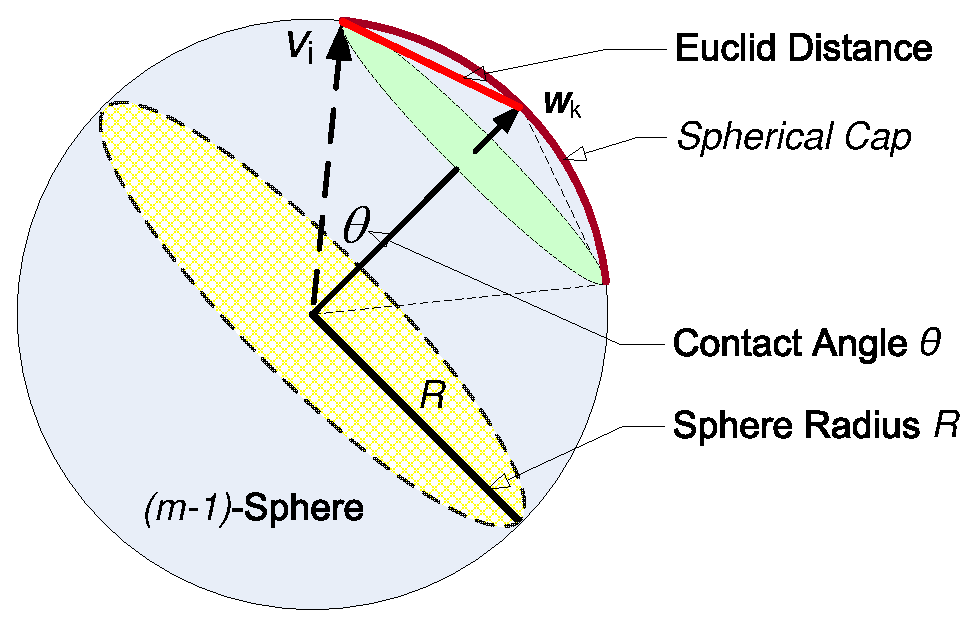
\includegraphics[width=1.80in, angle=0]{Sphere_Cap.eps}
\caption{Sphere and sphere cap}\label{Sphere_Cap} }
\end{figure}
\noindent With matching the sum area of the sphere-cap with the
sphere area, the boundary of a Voronoi cell can be approximated by
a hypershpere or a closed space curve defined in the following
proposition.
\begin{Prop}\label{approx_bound}(Hamming Boundary) The boundary of the uniform complex Voronoi cell $\bcV_{k}$ can be
approximated by a $(M-1)$-unit complex sphere or a closed complex
space curve.
\begin{equation}\hspace{-0.05in}
\begin{array}{rcl}
\bB\left(\bcV_{k}\right)&\approx& \bcS_{M}^{\rm c}(1)\bigcap \bcL_{M}^{\rm c}(\bw_{k},\ \cos(\theta)) \\
&=&\left\{\bv:\ \left\|\bv\right\|=1,\ \angle\left(\bv,\
\bw_{k}\right)=\theta\right\}\ ,
\end{array}
\end{equation}
\noindent where $\bcL_{M}^{\rm c}\left(\bw_{k},\
\cos(\theta)\right)=\left\{\bv:\ \bv^{\rm
H}\bw_{k}=\cos(\theta)\right\}$ denotes a complex space curve and
$\theta$ is
\begin{equation}%\hspace{-0.00in}
\begin{array}{rcl}
\theta&=&\arccos\left(\alpha_{0}\right)
\end{array}
\end{equation}
\noindent with
\begin{equation}\hspace{-0.00in}
\begin{array}{rcl}
\alpha_{0}&=&\left(\frac{2^B-1}{2^B}\right)^{\frac{1}{2M-2}}
\end{array}
\end{equation}
\noindent denoting the maximum loss ratio for antenna gain due to
channel quanitization.
\end{Prop}
On the other hand, if the ideal channel precoding vector $\bv_{i}$ is assumed to be a random variable of $M$-dimensional uniform distribution, the probability density
function (PDF) $\mbox{pr}\left(\alpha\right)$ and the cumulated
density function (CDF) $\mbox{Pr}\left(\alpha\right)$ of $\alpha$
are
\begin{equation}\hspace{-0.10in}
\begin{array}{rcl}
\mbox{pr}\left(\alpha\right)&=&\mbox{Prob}\left\{x=\alpha\right\}\\
&=&\begin{cases}
0 & 0\leq \alpha < \alpha_{0} \\
\frac{\left(2M-2\right)\alpha\left(1-\alpha^2\right)^{M-2}}{\left(1-\alpha_{0}^{2}\right)^{M-1}}
& \alpha_{0}\leq\alpha\leq 1
\end{cases}
\end{array}
\end{equation}
\noindent and
\begin{equation}\hspace{-0.10in}
\begin{array}{rcl}
\mbox{Pr}\left(\alpha\right)&=&\mbox{Prob}\left\{x\leq\alpha\right\} \\
&=&
\begin{cases}
0 & 0 \leq\alpha < \alpha_{0} \\
1-\left(\frac{1-\alpha^2}{1-\alpha_{0}^2}\right)^{M-1} &
\alpha_{0}\leq\alpha\leq 1
\end{cases}\ .
\end{array}
\end{equation}
\noindent With the assumption of uniform random codebook and
channel, the average received SINR $\bar\rho_{i}$ can be
lower-bounded by the following conclusion.
\begin{lemma} A heuristic mean of $\rho_{i}$
can be expressed by
\begin{equation}%\hspace{-0.10in}
\begin{array}{rcl}
\bar\rho_{i}&\approx&\frac{\sigma_{\alpha}^{2}\rho_{i}}{1+
\left(\frac{1-\sigma_{\alpha}}{M-1}\right)^{2}\sum\limits_{j\neq
i}\frac{\lambda_{i}}{\lambda_{j}}\rho_{j}}\ ,
\end{array}
\end{equation}
\noindent where  $\sigma_{\alpha}$ denotes the standard deviation
of $\alpha$ and $\sigma_{\alpha}^2$ is given by
\begin{equation}
\begin{array}{rcl}
\sigma_{\alpha}^2&=&\mbox{E}\left\{\alpha_{i}^2\right\}\\
&=&\int\limits_{1}^{\alpha_{0}}\frac{\left(2M-2\right)\alpha^3\left(1-\alpha^2\right)^{M-2}}{\left(1-\alpha_{0}^{2}\right)^{M-1}}d\alpha\\
&=&\frac{1}{M}+\frac{M-1}{M}\alpha_{0}^2\ .
\end{array}
\end{equation}
\end{lemma}

\section{Cramer-Rao Bound on Channel Estimat.}
In previous discussions, neither inter-symbol interference (ISI)
nor channel estimation is assumed. In general, the channel
estimation model for frequency-selective block fading channel is
different to (\ref{Direct_MIMO}). In channel estimation, not only
the whole channel impulse response but also the pilot placement
should be considered. Considering a $M$-input and $N$-output
channel with frequency-selective block fading, which means the
random channels taps remain constant for some data packets and
change to independent values for the next, the received baseband
signal can be written by
\begin{equation}\hspace{-0.20in}
\begin{array}{rcl}
\by(t)&=&\left[\begin{matrix}y_{1}(t)&y_{2}(t)&\cdots&y_{N}(t)\end{matrix}\right]^{\rm T}\\
&=&\left[\begin{matrix}\sum\limits_{m=1}^{M}h_{m,1}(t)\otimes s_m(t)\\ \sum\limits_{m=1}^{M}h_{m,2}(t)\otimes s_m(t)\\ \vdots \\
\sum\limits_{m=1}^{M}h_{m,N}(t)\otimes
s_m(t)\end{matrix}\right]+\left[\begin{matrix}n_{1}(t)\\ n_{2}(t)\\ \vdots\\
n_{N}(t)\end{matrix}\right]
\end{array}
\end{equation}
\noindent where  for  is the channel impulse response vector from
the $m$th transmit antenna to the $N$ receive antennas and
$s_m(t)$ denotes the transmitted symbol from the $m$th antenna.
Due to the commutativity of convolution, the stretched discrete
received signal vector could as well be expressed by the following
expression
\begin{equation}%\hspace{-0.00in}
\begin{array}{rcl}
\by&=&\bS\bh+\bn
\end{array},
\end{equation}
\noindent where $\bh$ is the stretched channel vector defined by
\begin{equation}\hspace{-0.00in}
\begin{array}{rcl}
\bh&=&\mbox{vec}\left(\left[\mbox{vec}(\bH_{1})\
\mbox{vec}(\bH_{2})\ \ldots\ \mbox{vec}(\bH_{N})\right]\right)
\end{array}
\end{equation}
\noindent with $\bH_{n}=\left[\bh_{n}(0)\ \bh_{n}(1)\ \ldots\
\bh_{n}(L_{c}-1)\right]$ and $\bh_{n}(l)=\left[h_{n,1}(l)\
h_{n,2}(l)\ \ldots\ h_{n,M}(l)\right]^{\rm T}$ for $1\leq l \leq
L_{c}$, and
\begin{equation}\hspace{-0.00in}
\begin{array}{rcl}
\bS&=&\mbox{kron}\left(\left[\bS_{1}\ \bS_{2}\ \ldots\
\bS_{M}\right]^{\rm T},\ \bI\right)
\end{array}
\end{equation}
\noindent with
\begin{equation}\hspace{-0.10in}
\begin{array}{rcl}
\bS_{k}&=&\left[\begin{matrix}
s_{k}(L)&\cdots&s_{k}(L-L_{c})\\
s_{k}(L-1)&\cdots&s_{k}(L-L_{c}-1)\\
\vdots&\ddots&\vdots\\
s_{k}(1)&\cdots&s_{k}(1-L_{c})
\end{matrix}\right]
\end{array}.\label{S_k}
\end{equation}
\noindent $L_{c}$ is the maximum channel order for all
subchannels. After the channel response vector $\bh$ is estimated,
we can calculate the channel correlation matrix $\bR_{\bH}$ by
\begin{equation}\hspace{-0.1in}
\begin{array}{rcl}
\hat{\bR}_{\bH}&=&\frac{1}{L_{c}}\sum\limits_{l=1}^{L_{c}}\sum\limits_{n=1}^{N}\bh_{n}\left(L_{c}+l\right)\bh_{n}^{\rm
H}\left(L_{c}+l\right)
\end{array}.\label{R_h_actual}
\end{equation}
\noindent There are many ways to put pilot symbols and data
symbols together for transmission. We focus on two most popular
designs: {orthogonal design} by {time-multiplexed pilot pattern},
and {non-orthogonal design} by {superimposed pilot pattern}.
\subsubsection{Time-Multiplexed Pilots and Data}
The concept of TMP design is to send $Q$ known pilot symbols and
$\left(L-Q\right)$ data symbols consecutively and separately in
time domain. One possible example of TMP is shown in
Fig.~\ref{pilot_pattern}(a), where the transmitted symbol
$s_{k}(l)$ becomes
\begin{equation}
\begin{array}{rcl}
s_{k}\left(l\right)&=&
\begin{cases}
s_{pk}(l) & 1 \leq l \leq Q \\
s_{dk}(l-Q) & Q+1\leq l\leq L
\end{cases}
\end{array},\label{TMP_k}
\end{equation}
\noindent where $s_{pk}(t)$, $1\leq t \leq Q$, denotes the pilot
symbols transmitted in power $\sigma_{p}^2$ and $s_{dk}(t)$,
$Q+1\leq t \leq L$, denotes the data symbols transmitted in power
$\sigma_{d}^2$.
\subsubsection{Superimposed Pilots and Data}
In SIP design, data symbols and pilot symbols are simultaneously
sent within one frame of $L$ symbols. This can be shown in
Fig.~\ref{pilot_pattern}(b). In this case, the transmitted symbol
$s_{k}(l)$ becomes
\begin{equation}
\begin{array}{rcl}
s_{k}\left(l\right)&=&\frac{\sigma_{p}}{P}s_{pk}\left(l\right)+\frac{\sigma_{d}}{P}s_{dk}\left(l\right)\
,\ 1\leq l\leq L\ ,
\end{array}\label{SIP_k}
\end{equation}
\noindent with $\sigma_{p}^2+\sigma_{d}^2=P$.

The lower bound to the mean-squared errors (MSE) of unbiased
channel estimates is given by CRLB, which is defined as the
inverse of the Fisher Information Matrix (FIM). If we denotes
$\bvartheta=\left[\bh^{\rm T}\ \bs_{d}^{\rm T}\right]^{\rm T}$,
the complex FIM is given by
\begin{equation}\hspace{-0.10in}
\begin{array}{rcl}
\mbox{F}\left(\bvartheta\right)&=&\mbox{E}\left\{\left[\frac{\partial\ln\mbox{Pr}\left(\by|\vartheta\right)}{{\partial\vartheta}^{\ast}}\right]\left[\frac{\partial\ln\mbox{Pr}\left(\by|\vartheta\right)}{{\partial\vartheta}^{\ast}}\right]^{\rm H}\right\}\\
 &\hspace{-0.90in}=&\hspace{-0.50in}\sigma_{n}^{-2}\left[\begin{matrix}
\mbox{E}\left\{\bS^{\rm
H}\bS\right\}+\rho_{h}^2\bI&\bzero\\
\bzero&\mbox{E}\left\{\bcH^{\rm H}\bcH\right\}+\rho_{s_{d}}^2\bI
\end{matrix}\right]\ ,
\end{array}\label{FIM}
\end{equation}
\noindent where
$\rho_{h}^{2}=\mbox{E}\left\{\left|\frac{\partial\ln\mbox{Pr}\left(h\right)}{{\partial
h}^{\ast}}\right|^2\right\}$ and
$\rho_{s_{d}}^{2}=\mbox{E}\left\{\left|\frac{\partial\ln\mbox{Pr}\left(s_{d}\right)}{{\partial
s_{d}}^{\ast}}\right|^2\right\}$. With (\ref{FIM}), the MSE of the
estimates of $\bR_{\bh}=\bh\bh^{\rm H}$ is then given by
\begin{equation}
\begin{array}{rcl}
\mbox{MSE}\left\{\bR_{\bh}\right\}&=&\sigma_{n}^{2}\left[\mbox{E}\left\{\bS^{\rm
H}\bS\right\}+\rho_{h}^2\bI\right]^{-1}
\end{array}.
\end{equation}
\noindent The CRLB on the channel estimation with either TMP or
SIP can therefore be formulated by the following lemma.
\begin{lemma}(Cramer-Rao Lower Bound) For the time-multiplexed pilot and data design defined in
(\ref{TMP_k}), the CRLB of channel estimation is
\begin{equation}
\begin{array}{rcl}
\varepsilon_{h}^{\rm
TMP}&\geq&\left[\rho_{h}^2+Q\rho_{p}^2+\left(L-Q\right)\rho_{d}^2\right]^{-1}
\end{array}.\label{CRLB_TMP}
\end{equation}
\noindent For the superimposed pilot and data design defined in
(\ref{SIP_k}), the CRLB of channel estimation is
\begin{equation}\
\begin{array}{rcl}
\varepsilon_{h}^{\rm
SIP}&\geq&\left[\rho_{h}^2+L\left(\rho_{p}^2+\rho_{d}^2\right)\right]^{-1}
\end{array}\label{CRLB_SIP}
\end{equation}
\noindent where $\rho_{p}^2=\frac{\sigma_{p}^2}{\sigma_{n}^2}$
denotes the SNR of received pilot signals and
$\rho_{d}^2=\frac{\sigma_{d}^2}{\sigma_{n}^2}$ denotes the SNR of
received data signals.
\end{lemma}
Now if we look back at (\ref{R_h_actual}), with the assumptions
that the channel is constant during estimation, pilots and data
are random and independent to each and an optimal channel
estimation is done by receiver, a heuristic view of the MIMO
channel correlation matrix can be written by
\begin{equation}
\begin{array}{rcl}
\hat{\bR}_{\bH}&\approx&\bR_{\bH}+\frac{\varepsilon_{h}}{\sqrt{L_{c}N}}\bI_{M}
\end{array},\label{R_h_approx}
\end{equation}
\noindent where $\varepsilon_{h}$ denotes the MSE of channel
estimates, which can be either $\varepsilon_{h}^{\rm TMP}$ or
$\varepsilon_{h}^{\rm SIP}$. With (\ref{R_h_approx}), it shows
that the channel estimation error at the receiver side will mostly
affect the accuracy of the eigenvalues estimated by the receiver.
The MSE of eigenvalue estimates is then bounded by
\begin{equation}
\begin{array}{rcl}
\varepsilon_{\lambda}&\gtrsim&\frac{\varepsilon_{h}}{\sqrt{L_{c}N}}
\end{array}.\label{eigenvalue_bound}
\end{equation}
There are two major effects of PAT on MIMO channel throughput. The
first one is that pilot itself will take away channel resources
from data transmission. The second one is that it may affect the
transmit power allocation. If orthogonal pilot pattern is used,
there will be linearly degradation on channel throughput so that
\begin{equation}%\hspace{-0.2in}
\begin{array}{rcl}
\eta_{\rm TM}& =&\frac{L-Q}{L}
\sum\limits_{k=1}^{K}\log\left(1+\frac{\hat{\rho}_{i}}{M}\right)
\end{array},\label{spectral_eff_TM}
\end{equation}
\noindent where $\hat{\rho}_{i}$ denotes the suboptimal power
allocation due to channel estimation error, and if superimposed pilot
pattern is employed, the MIMO throughput will become
\begin{equation}%\hspace{-0.2in}
\begin{array}{rcl}
\eta_{\rm
SI}&=&\sum\limits_{k=1}^{K}\log\left(1+\frac{\sigma_{d}^{2}}{P}\frac{\hat{\rho}_{i}}{M}\right)
\end{array},\label{spectral_eff_SI}
\end{equation}
\noindent even though ideal beamforming vectors $\bv_{k}$, $k=1,\ 2,\ \ldots,\ K$, are available at the transmitter side.

\section{Multi-Antenna Relay Network}
In order to understand the asymptotic behavior of MIMO beamforming
with channel estimation and quantization, a multi-hop
amplify-and-forward MIMO relay network is considered. Without loss
of generality, we assume that every relay station has $M$ transmit
antennas and $N$ receive antennas, every MIMO link is uniform
random and independent to each other with same pilot pattern and
the same codebook is shared in the network. The end-to-end average
throughput for MIMO relay link with $G$ hops roughly is
\begin{equation}\hspace{-0.15in}
\begin{array}{rcl}
\bar\eta_{\rm
TM}&\approx&\frac{(L-Q)K}{L}\log\left[1+\frac{\rho}{M}\left(\frac{\sigma_{\alpha}^{2}}{1+\frac{(1-\sigma_{\alpha})^2}{M-1}\rho}\right)^{G}\right]
\end{array}\label{RN_TM}
\end{equation}
\noindent if tim-multiplexed pilot pattern is used, or
\begin{equation}\hspace{-0.23in}
\begin{array}{rcl}
\bar\eta_{\rm
SI}&\approx&K\log\left[1+\frac{\sigma_{d}^{2}\rho}{PM}\left(\frac{\sigma_{\alpha}^{2}}{1+\frac{(1-\sigma_{\alpha})^2}{M-1}\rho}\right)^{G}\right]
\end{array}\label{RN_SI}
\end{equation}
\noindent if superimposed pilot pattern is used, where
$\rho=\mbox{E}\{\rho_{k}\}$ denotes the average received SNR for
each MIMO beam. If we consider the performance of multi-antenna
relay network in high SNR region where IBI is the dominant factor
affecting end-to-end throughput, (\ref{RN_TM}) becomes
\begin{equation}\hspace{-0.18in}
\begin{array}{l}
\bar\eta_{\rm
TM}\approx\frac{(L-Q)K}{L}\log\left[1+\frac{(M-1)^{G}}{M\rho^{G-1}}\left(\frac{\sigma_{\alpha}}{1-\sigma_{\alpha}}\right)^{2G}\right]
\end{array}\label{RN_TM_high_SNR}
\end{equation}
\noindent and (\ref{RN_SI}) becomes
\begin{equation}\hspace{-0.23in}
\begin{array}{rcl}
\bar\eta_{\rm
SI}&\approx&K\log\left[1+\frac{\sigma_{d}^{2}}{P}\frac{(M-1)^{G}}{M\rho^{G-1}}\left(\frac{\sigma_{\alpha}}{1-\sigma_{\alpha}}\right)^{2G}\right]
\end{array}.\label{RN_SI_high_SNR}
\end{equation}
With (\ref{RN_TM_high_SNR}) and (\ref{RN_SI_high_SNR}), it shows
that the end-to-end throughput in high SNR region of MIMO relay
network with channel estimation and quantization actually will
decrease even though increasing transmit signal power in each hop.
The network capacity becomes interference-limited.
\section{Conclusions}
In this paper, the Hamming boundary for the Voronoi decomposition
of uniform random codebook and the SINR of beamforming with
channel quantization are formulated. And the effects of imperfect
channel estimation with either time-multiplexed pilot pattern or
superimposed pilot pattern on MIMO beamforming is discussed.
Finally the scalability of MIMO beamforming relay network with
imperfect channel estimation and quantization is discussed.
\small
\bibliographystyle{unsrt}
\bibliography{Cooperative_Relay}
\end{document}
